
\section{原材料的订购和转运方案扩展}

本题要求在尽量多地采购A类和尽量少地采购C类原材料的前提下,制定最经济的原材料订购方案和损耗最小的转运方案,并分析方案的实施效果。

\subsection{制定订购方案}

该企产为了压缩生产成本,要减少转运及仓储的成本。
三类原材料运输和业为了压缩生存储的单位费用相同,但A类原材料的商品生产能力比C类原材料强,因此企业会尽量多地采购A类和尽量少地采购C类原材料。
本文忽略了原材料类型偏好对每周订货总量的影响,而主要关注于供应商订购量分配的变化。
因此,问题2中的每周订货总量计划保持不变。

问题2中,原材料的订购数量是直接根据供应商的评价来进行分配的。
问题1中建立的评价模型并未重点关注供应商贩卖的原材料类型,本文通过依据供应商贩卖的原材料类型,对供应商的评价加分,以尽量多地采购A类和尽量少地采购C类原材料。
考虑到综合评价指标均小于1分,本文对售卖A类原材料的供应商加1分,令企业尽量多地采购A类原材料。
联系上文,B类原材料的本征采购单价实际上略高,因此,本文没有对C类原材料的供应商扣分。

\subsection{制定运输方案}

因为A类原材料的采购单价较高,因此对转运损耗更加敏感。
问题3中企业计划尽量多地采购A类原材料,所以迫切需要制定合理的运输方案,以确保转运商的转运损耗率尽量少,来达到压缩生产成本的目的。
问题2中侧重于经济效益,要求损耗最少,而问题3要求转运损耗率尽量少,因此对问题2中的0$\textendash$1规划模型稍加改动:

\begin{equation}
\begin{array}{l}
\min \sum_{l=1}^{8}\left(\iota_{l} \sum_{j=1}^{44} \rho_{i j l} \psi_{i j}\right) \\
\text { s.t. }\left\{\begin{array}{l}
\sum_{i=1}^{8} \rho_{i j l}=1 \\
\sum_{j=1}^{44} \rho_{i j l} \psi i_{i j} \leq 6000
\end{array}\right.
\end{array}
\end{equation}

式中$L'_i$代表第$i$周的转运损耗量,由于希望转运损耗率尽量少,故此处转运损耗量应取最小值。

\subsection{仿真模拟分析方案实施效果}

仿照问题2,此处本文也进行了仿真模拟,绘制了企业仓库储存量随周数的变化情况关系,如下图9所示:

\begin{center} {\centering
\vbox{
	\centerline{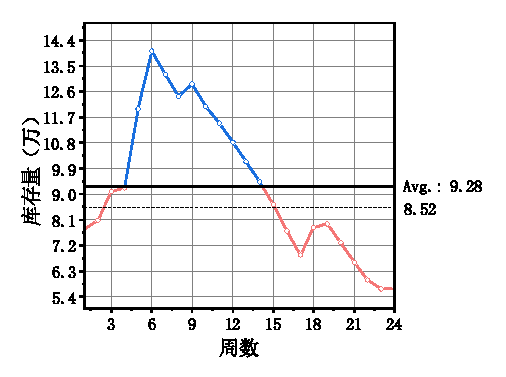
\includegraphics[width=8cm]{Image/qus_3_库存.eps}}
	\vskip 1mm{\small
	图9\quad 企业库存量变化.\label{lstm}
	\\}
	}
	}
\end{center}

由图可知,在问题2的基础上库存量总体向下平移,节约了仓储费用,模型效果显著。
相比问题2,此处调高了仓储成本与采购单价或售价之比,符合现实中企业偏爱A类原材料的原因,这也使企业的囤货倾向有所收敛。

